\documentclass[../main.tex]{subfiles}
\graphicspath{{\subfix{../figures/}}}
%
\begin{document}
\section{享元模式(Flyweight)}
\textbf{享元模式的用意}:
享元模式是对象的结构模式. 享元模式以共享的方式高效地支持大量的细粒度对象的维护与管理.
享元对象能实现共享的关键是区分\textbf{内部状态}(Internal  state)和\textbf{外部状态}(External State).

当以下所有条件都满足时,可以考虑使用享元模式:
\begin{enumerate}
  \item 一个系统有大量的对象.
  \item 这些对象消耗大量的内存.
  \item 这些对象的状态中的大部分都可以外部化.
  \item 软件系统不依赖于这些对象的身份,即这些对象可以是不可分辨的.
\end{enumerate}
%
\textbf{内部状态}是存储在享元对象内部的并且是不会随环境改变而有所不同的.因此,一个享元可以具有内部状态并可以共享.

\textbf{外部状态}是随环境改变而改变的、不可以共享的状态.享元对象的外部状态必须由客户端保存,并在享元对象被创建之后,在需要使用的时候再传入到享元对象内部.
外部状态不可以影响享元对象的内部状态.内外部状态是互相独立的.

\textbf{享元模式的种类}:
根据所涉及的享元对象的内部结构,享元模式可以分成\textbf{单纯享元模式}
和\textbf{复合享元模式}两种形式.下图是单纯享元模式的结构示意图:
%
\begin{figure}[H]
  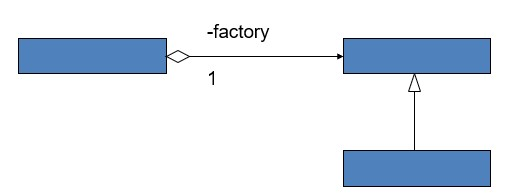
\includegraphics[width=0.45\textwidth]{24_1.jpg}
\end{figure}
%
下图所示是复合享元模式的结构示意图:
%
\begin{figure}[H]
  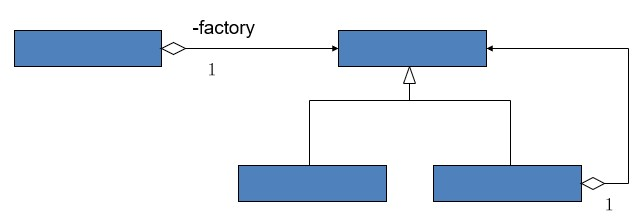
\includegraphics[width=0.45\textwidth]{24_2.jpg}
\end{figure}
%
可见,在复合享元模式中,享元对象构成合成模式.因此,\textbf{复合享元模式}实际上是\textbf{单纯享元模式}与\textbf{合成模式}的组合.

\textbf{享元模式的应用}:
\begin{itemize}
  \item 享元模式在编辑器系统中大量使用.一个文本编辑器往往会提供很多种字体,而通常的做法就是将每一个字母作成一个享元对象.享元对象的内部状态就是这个字母的字符数据,而字母在文本中的位置和字体风格等其它信息则是外部状态.
  \item 在Java语言中,String类型就使用了享元模式.String对象是不变对象,一旦创建出来就不能改变.
\end{itemize}
%
\subsection{单纯享元模式的结构}
\noindent 单纯享元模式中,所有享元对象都是可以共享的.下图是一个单纯享元模式的简单实现:
%
\begin{figure}[H]
  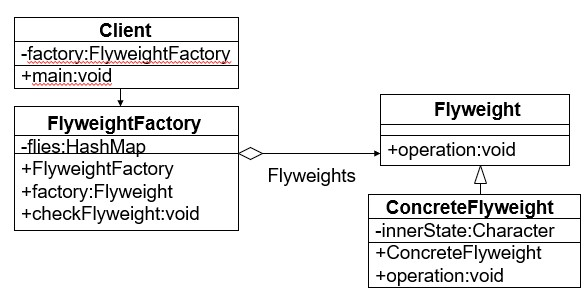
\includegraphics[width=0.55\textwidth]{24_3.jpg}
\end{figure}
%
\textbf{单纯享元模式涉及的角色}:
\begin{itemize}
  \item 抽象享元角色:该角色是所有的具体享元类的超类,为这些类规定出需要实现的公共接口.
  \item 具体享元(ConcreteFlyweight)角色:实现抽象享元角色所规定的接口.
  \item 享元工厂(FlyweightFactory)角色:本角色负责创建和管理享元角色
  \item 客户端(Client)角色:本角色需要维护一个对所有享元对象的引用.
\end{itemize}
%
\lstinputlisting[language=java]{./code/24/1/Flyweight.java}
\lstinputlisting[language=java]{./code/24/1/ConcreteFlyweight.java}
%
客户端不可以直接将具体享元类实例化,而必须通过一个工厂对象,利用一个factory()方法得到享元对象.一般而言,享元对象在整个系统中只有一个,因此可以使用单例模式.
当客户端需要单纯享元对象的时候,需要调用享元工厂的factory()方法,并传入所需的单纯享元对象的内部状态.
%
\lstinputlisting[language=java]{./code/24/1/FlyweightFactory.java}
%
\subsection{复合享元模式的结构}
在上面的单纯享元模式中,所有的享元对象都是单纯享元对象,即都是可以直接共享的.下面考虑一个较复杂的情况,将一些单纯享元使用合成模式加以组合,形成复合享元对象.这样的复合本身不能共享,但是它们可以分解成单纯享元对象,而后者可以共享.
复合享元模式的类图如下:
%
\begin{figure}[H]
  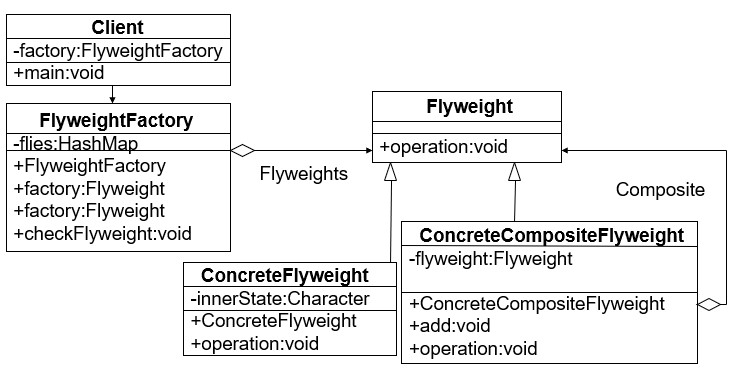
\includegraphics[width=0.75\textwidth]{24_4.jpg}
\end{figure}
%
\textbf{复合享元模式涉及的角色}:
\begin{itemize}
  \item 抽象享元角色:此角色是所有的具体享元类的超类,为这些类规定出需要实现的公共接口.
  \item 具体享元(ConcreteFlyweight)角色:实现抽象享元角色所规定的接口.
  \item 复合享元(UnsharableFlyweight)角色:复合享元角色所代表的对象是不可以共享的,但是一个复合享元对象可以分解成为多个本身是单纯享元对象的组合.
  \item 享元工厂(FlyweightFactory)角色:负责创建和管理享元角色.必须保证享元对象可以被系统适当的地共享.
  \item 客户端(Client)角色:使用享元对象,但需要自行存储所有享元对象的外部状态.
\end{itemize}
%
\lstinputlisting[language=java]{./code/24/2/Flyweight.java}
%
\textbf{具体享元角色的主要责任}:
\begin{itemize}
  \item 实现了抽象享元角色所声明的接口,也就是operation()方法.Operation()方法接收外部状态作为参数.
  \item 为内部状态提供存储空间的,在本实现中就是innerState属性.享元模式本身对内部状态的存储类型并无要求,这里的内部状态就是Character类型,是为了给复合享元的内部状态选做String类提供方便.
\end{itemize}
%
\lstinputlisting[language=java]{./code/24/2/ConcreteFlyweight.java}
%
\lstinputlisting[language=java]{./code/24/2/ConcreteCompositeFlyweight.java}
%
当客户端需要复合享元对象的时候,需要调用享元工厂的factory()方法,并传入所需的复合享元对象的所有复合元素的内部状态.
\lstinputlisting[language=java]{./code/24/2/FlyweightFactory.java}
%
\subsection{单例模式实现享元工厂角色}
系统往往只需要一个享元工厂的实例,所以享元工厂可以设计成为单例模式.

单纯享元模式中的享元工厂角色:
%
\begin{figure}[H]
  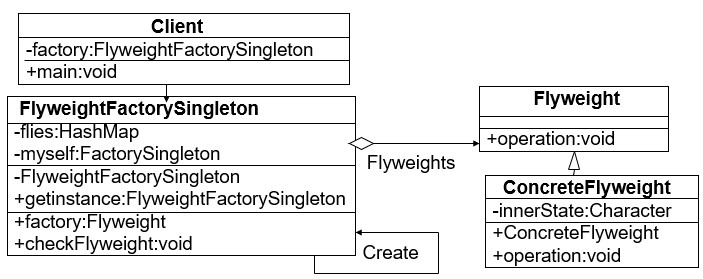
\includegraphics[width=0.75\textwidth]{24_5.jpg}
\end{figure}
%
这是一个示意性客户端类的源代码,显示出调用单例工厂对象的getInstance()方法,以得到具体享元类.
%
\lstinputlisting[language=java]{./code/24/3/ClientSingleton.java}
%
\subsection{例子:户外咖啡摊}
\textbf{系统的要求}:
在这个咖啡摊(Coffee Stall)所使用的系统里,有一系列具有不同``口味(Flavor)''的咖啡.
客人到摊位上购买咖啡,所有的咖啡均放在台子上,客人自己买到咖啡后就离开摊位.
咖啡有内部状态,也就是咖啡的口味;咖啡没有外部状态.
如果系统为每一杯咖啡都创建一个独立的对象那么就需要创建很多小对象,所以只要把咖啡按照种类(即口味)划分,
每一种口味的咖啡只创建一个对象,并实行共享.
%
\begin{figure}[H]
  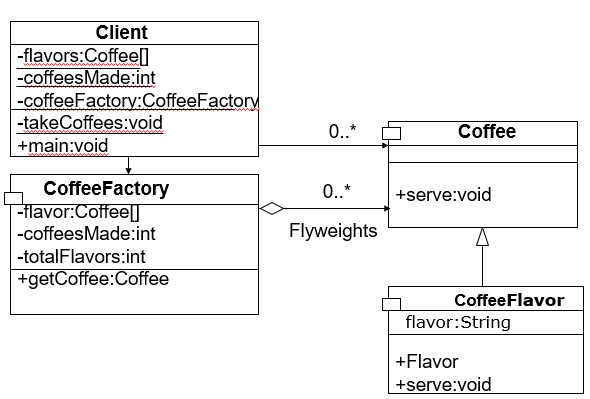
\includegraphics[width=0.75\textwidth]{24_6.jpg}
\end{figure}
%
在这里享元模式所涉及的角色如下:
\begin{itemize}
  \item 抽象享元(抽象咖啡)角色:此角色由Coffee类扮演,它是所有的具体享元类的超类,为这些类规定出需要实现的公共接口.
  \item 具体享元(不同``口味''的咖啡)角色:这个角色有CoffeeFlavor类扮演,它的实例是可以共享的.每一个不同的咖啡都对应于独立而且唯一的享元对象.
  \item 享元工厂(咖啡工厂)角色:这个角色由CoffeeFactory类扮演,它负责创建所有``口味''的咖啡对象.
\end{itemize}
%
客户端并不直接创建任何``口味''的咖啡对象,而是向咖啡工厂提出请求,由咖啡工厂提高一个相应的对象.
下面是抽象享元角色的源代码:
%
\lstinputlisting[language=java]{./code/24/4/Coffee.java}
%
``口味''角色的源代码实现了抽象Order角色所声明的接口:
%
\lstinputlisting[language=java]{./code/24/4/CoffeeFlavor.java}
%
所有不同``口味''的咖啡对象都应当由咖啡工厂提供,而不应当由客户端直接创建.咖啡工厂的源代码如下:
%
\lstinputlisting[language=java]{./code/24/4/CoffeeFactory.java}
%
下面是系统的客户端角色的源代码,该角色可代表咖啡摊的工作人员.
%
\lstinputlisting[language=java]{./code/24/4/Client.java}
%
可以看出,这个咖啡摊可以为客人准备最多20种不同口味的咖啡.虽然上面的客户端对象叫了11杯咖啡,但是所有咖啡的口味却只有三种,即Capucino、Espresso和Black Coffee.
%
\subsection{例子:咖啡屋}
\textbf{系统的要求}:
在前面的咖啡摊项目里,由于没有供客人坐的桌子,所有的咖啡对象均没有考虑环境的影响.咖啡仅有内部状态,也就是咖啡的种类,而没有外部状态.
下面考虑一个规模稍稍大一点的咖啡屋(Coffee Shop)项目.屋子里有很多桌子供客人坐,系统除了需要提供不同``口味''的咖啡之外,还需要跟踪咖啡被送到哪一个桌位上,因此,咖啡就有了桌子作为外部状态.

\textbf{系统的设计}:
由于外部状态的存在,没有外部状态的单纯享元模式不再符合要求.系统的设计可以利用有外部状态的单纯享元模式.
在这里享元模式所涉及的角色与咖啡摊项目的角色都是一样的,除了Table角色之外:
\begin{itemize}
  \item 环境角色:由Table类扮演,这就是所有的享元角色所涉及的外部状态.
  \item 抽象享元角色:此角色由Coffee类扮演,它是所有的具体享元类的超类,为这些类规定出需要实现的公共接口.
  \item 具体享元(咖啡``口味'')角色: 该角色由CoffeeFlavor类扮演,它的实例是可以共享的.每一杯不同的咖啡都对应一个独立而且唯一的享元对象.一个咖啡对象在创建出来之后,其内部状态就不再改变.
  \item 享元工厂角色:该角色由FlavorFactory类扮演,它负责创建一个对应的咖啡对象.在客户端提出请求后,咖啡工厂就会检查是否已经有一个对应的对象存在,如已有,直接返回这个已有的对象;反之,创建一个新的对象,并提供给客户端.
  \item 客户端(Client)角色:客户端并不直接创建任何``口味''的咖啡对象,而是向咖啡工厂提出请求,由咖啡工厂提供一个相应的对象.本角色代表咖啡屋的负责招待客人的侍者,侍者代替客人向调制咖啡的工作人员请求咖啡,后者将调制好的咖啡提供给侍者.
\end{itemize}
%
\begin{figure}[H]
  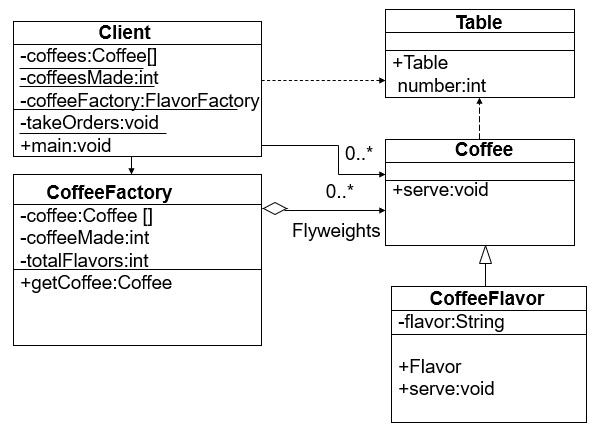
\includegraphics[width=0.75\textwidth]{24_7.jpg}
\end{figure}
%
抽象享元角色的源代码如下:
%
\lstinputlisting[language=java]{./code/24/5/Coffee.java}
%
``口味''角色的源代码如下:
%
\lstinputlisting[language=java]{./code/24/5/CoffeeFlavor.java}
%
``口味''工厂的源代码:
%
\lstinputlisting[language=java]{./code/24/5/CoffeeFactory.java}
%
系统环境角色Table类的代码:
%
\lstinputlisting[language=java]{./code/24/5/Table.java}
%
系统客户端角色代码如下:
%
\lstinputlisting[language=java]{./code/24/5/Client.java}
%
\end{document}
